\documentclass{beamer}
\usetheme{Boadilla}

\usepackage{tikz}
\usetikzlibrary{shapes}

\usepackage{multicol}

\title{Git Gud}
\author{Neil Ashford}
\institute{UQ Computing Society}
\date{2018-04-23T17:30+10:00}

\AtBeginSection[]
{
    \begin{frame}
        \frametitle{Outline}
        \begin{multicols}{2}
            \tableofcontents[currentsection]
        \end{multicols}
    \end{frame}
}

\begin{document}

\begin{frame}
    \titlepage
\end{frame}

\section{Introduction}

\subsection{Who am I}
\begin{frame}
    \frametitle{Who am I}
    \begin{itemize}[<+->]
        \item Neil Ashford
        \item 4th year Software\only<2->{\footnote{ish}} Engineering
        \item Committee member
        \item \textbf{@artemis} on slack, \url{ashfordneil0@gmail.com}
        \item Tutor for CSSE2002, CSSE2010 and CSSE2310
    \end{itemize}
\end{frame}

\subsection{What is this talk}
\begin{frame}
    \frametitle{What is this talk}
    Target Audience
    \pause
    \begin{itemize}[<+->]
        \item People who have never used version control.
        \item People who have ``memorised 5 shell commands and trust them implicitly without understanding''
    \end{itemize}
    \pause
    What I'll Cover
    \begin{itemize}[<+->]
        \item Some really basic version control you're familiar with, and its flaws.
        \item The pieces of a mental model of proper version control.
        \item How git represents each of those pieces to you.
        \item Flaws with git, and alternatives.
    \end{itemize}
    \pause
    What I Won't Cover
    \begin{itemize}[<+->]
        \item How to \textbf{cheat} when using git
    \end{itemize}
\end{frame}

\section{The Version Control We Know}

\subsection{Meet the Culprit}
\begin{frame}
    \frametitle{Meet the Culprit}
    \begin{itemize}[<+->]
        \item Live demos suck, so we're trying to stick with something familiar.
        \item Please welcome our old friend...
        \item Microsoft Word\only<3->{\footnote{Okay I'm on a mac so it's pages but still}}
    \end{itemize}
\end{frame}

\subsection{Undo / Reverts}
\begin{frame}
    \frametitle{Undo / Reverts}

    \begin{columns}
        \begin{column}{0.5\textwidth}
            \begin{itemize}[<+->]
                    \pause
                \item Type ``Hello''
                \item Type ``World''
                \item Type ``Filler Text''
                \item Press Undo
                \item Press Redo
                \item Press Undo again
            \end{itemize}
        \end{column}
        \begin{column}{0.5\textwidth}
            \begin{tikzpicture}
                \only<2->{
                    \node[circle, draw, minimum size=1cm] (A) at (0,0) {Hello};
                }
                \only<3->{
                    \node[circle, draw, minimum size=1cm] (B) at (0,-2) {World};
                    \draw[->] (A) -- (B);
                }
                \only<4,6>{
                    \node[circle, draw, minimum size=1cm] (C) at (0,-4) {Filler Text};
                    \draw [->] (B) -- (C);
                }
                \only<5,7>{
                    \node[gray, dashed, circle, draw, minimum size=1cm] (C) at (0,-4) {Filler Text};
                    \draw [gray, dashed, ->] (B) -- (C);
                }
            \end{tikzpicture}
        \end{column}
    \end{columns}
\end{frame}

\subsection{Branches}
\begin{frame}
    \frametitle{Branches}

    \begin{columns}
        \begin{column}{0.5\textwidth}
            \begin{itemize}[<+->]
                \item From where we were before...
                \item Type ``Lorem Ipsum''
                \item Realise we want ``Filler Text'' back
                \item Press Undo
                \item Press Redo
                \item Weep
            \end{itemize}
        \end{column}
        \begin{column}{0.5\textwidth}
            \begin{tikzpicture}
                \only<1->{
                    \node[circle, draw, minimum size=1cm] (A) at (0,0) {Hello};
                    \node[circle, draw, minimum size=1cm] (B) at (0,-2) {World};
                    \draw[->] (A) -- (B);
                }
                \only<1>{
                    \node[gray, dashed, circle, draw, minimum size=1cm] (C) at (0,-4) {Filler Text};
                    \draw[gray, dashed, ->] (B) -- (C);
                }
                \only<2->{
                    \node[red, dashed, circle, draw, minimum size=1cm] (C) at (0,-4) {Filler Text};
                    \draw[red, dashed, ->] (B) -- (C);
                }
                \only<2,3,5->{
                    \node[circle, draw, minimum size=1cm] (D) at (3,-4) {Lorem Ipsum};
                    \draw[->] (B) -- (D);
                }
                \only<4>{
                    \node[gray, dashed, circle, draw, minimum size=1cm] (D) at (3,-4) {Lorem Ipsum};
                    \draw[gray, dashed, ->] (B) -- (D);
                }
            \end{tikzpicture}
        \end{column}
    \end{columns}
\end{frame}

\subsection{Merges and Collaborative Work}
\begin{frame}
    \frametitle{Merges and Collaborative Work}

    \begin{columns}
        \begin{column}{0.5\textwidth}
            \begin{itemize}[<+->]
                \item From where we were before...
                \item Save it, throw it on a USB, give it to a friend
                \item \textbf{We} write ``dolor sit amet'' at the \textbf{end} of the document
                \item \textbf{They} write ``git is cool'' at the \textbf{top} of the document
                \item How to combine these?
            \end{itemize}
        \end{column}
        \begin{column}{0.5\textwidth}
            \resizebox{\textwidth}{!}{
                \begin{tikzpicture}
                    \only<1->{
                        \node[circle, draw, minimum size=1cm] (A) at (0,0) {Hello};
                        \node[circle, draw, minimum size=1cm] (B) at (0,-2) {World};
                        \draw[->] (A) -- (B);
                        \node[gray, dashed, circle, draw, minimum size=1cm] (C) at (0,-4) {Filler Text};
                        \draw[gray, dashed, ->] (B) -- (C);
                        \node[circle, draw, minimum size=1cm] (D) at (3,-4) {Lorem Ipsum};
                        \draw[->] (B) -- (D);
                    }
                    \only<3->{
                        \node[blue, circle, draw, minimum size=1cm] (E) at (3,-7) {dolor sit amet};
                        \draw[blue, ->] (D) -- (E);
                    }
                    \only<4->{
                        \node[green, circle, draw, minimum size=1cm] (F) at (6,-6) {git is cool};
                        \draw[green, ->] (D) -- (F);
                    }
                    \only<5>{
                        \node[circle, draw, minimum size=1cm] (G) at (4.5, -9) {merge};
                        \draw[->] (E) -- (G);
                        \draw[->] (F) -- (G);
                    }
                \end{tikzpicture}
            }
        \end{column}
    \end{columns}
\end{frame}

\section{A Git Mental Model}

\subsection{Differences Between Our Live Demo and Git}
\begin{frame}
    \frametitle{Differences Between Our Live Demo and Git}

    \begin{columns}
        \begin{column}{0.5\textwidth}
            \begin{itemize}[<+->]
                \item Microsoft Word can't do all of these things
                \item (Git can)
                \item Undo and Redo track really small changes in a single file
                \item Git tracks larger changes, in a directory (hereafter, repository)
                \item ...and more
            \end{itemize}
        \end{column}
        \begin{column}{0.5\textwidth}
            \resizebox{\textwidth}{!}{
                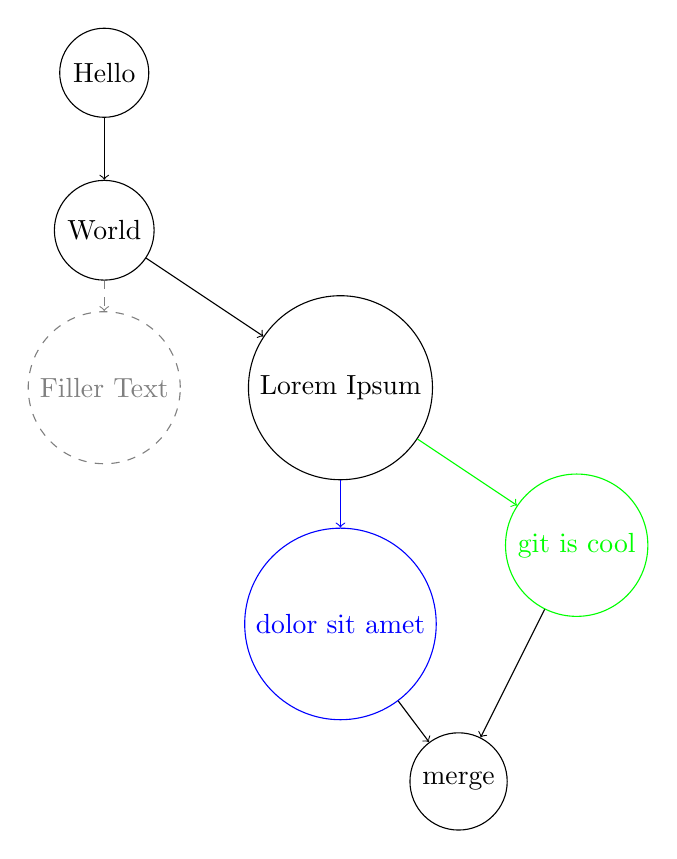
\begin{tikzpicture}
                    \node[circle, draw, minimum size=1cm] (A) at (0,0) {Hello};
                    \node[circle, draw, minimum size=1cm] (B) at (0,-2) {World};
                    \draw[->] (A) -- (B);
                    \node[gray, dashed, circle, draw, minimum size=1cm] (C) at (0,-4) {Filler Text};
                    \draw[gray, dashed, ->] (B) -- (C);
                    \node[circle, draw, minimum size=1cm] (D) at (3,-4) {Lorem Ipsum};
                    \draw[->] (B) -- (D);
                    \node[blue, circle, draw, minimum size=1cm] (E) at (3,-7) {dolor sit amet};
                    \draw[blue, ->] (D) -- (E);
                    \node[green, circle, draw, minimum size=1cm] (F) at (6,-6) {git is cool};
                    \draw[green, ->] (D) -- (F);
                    \node[circle, draw, minimum size=1cm] (G) at (4.5, -9) {merge};
                    \draw[->] (E) -- (G);
                    \draw[->] (F) -- (G);
                \end{tikzpicture}
            }
         \end{column}
    \end{columns}
\end{frame}

\subsection{Commits}
\begin{frame}
    \frametitle{Commits}

    \begin{columns}
        \begin{column}{0.5\textwidth}
            \begin{itemize}[<+->]
                \item The \textbf{atomic unit} of git
                \item You make the commits
                \item A commit consists of 3 things
                \item The state of the repo when that commit was made
                \item What commit(s) came immediately before it
                \item Metadata (timestamp, author, cryptographic hash)
            \end{itemize}
        \end{column}
        \begin{column}{0.5\textwidth}
            \begin{tikzpicture}
                \node[circle, draw, minimum size=5cm] (A) at (0,0) {Hello};
            \end{tikzpicture}
        \end{column}
    \end{columns}
\end{frame}

\subsection{Reverts}
\begin{frame}
    \frametitle{Reverts}

    \begin{columns}
        \begin{column}{0.5\textwidth}
            \begin{itemize}[<+->]
                \item Expressed in terms of commits
                \item Only appends to the history
                \item Can revert multiple commits at once
                \item Don't have to revert the most recent commit
            \end{itemize}
        \end{column}
        \begin{column}{0.5\textwidth}
            \resizebox{!}{0.8\textheight}{
                \begin{tikzpicture}
                    \only<1->{
                        \node[circle, draw, minimum size=1cm] (A) at (0,0) {Hello};
                        \node[circle, draw, minimum size=1cm] (B) at (0,-2) {World};
                        \draw[->] (A) -- (B);
                    }
                    \only<1>{
                        \node[gray, dashed, circle, draw, minimum size=1cm] (C) at (0,-4) {Filler Text};
                        \draw [gray, dashed, ->] (B) -- (C);
                    }
                    \only<2->{
                        \node[circle, draw, minimum size=1cm] (C) at (0,-4) {Filler Text};
                        \draw [->] (B) -- (C);
                        \node[circle, draw, minimum size=1cm] (C2) at (0,-7) {\texttt{remove} Filler Text};
                        \draw [->] (C) -- (C2);
                    }
                \end{tikzpicture}
            }
        \end{column}
    \end{columns}
\end{frame}

\subsection{Branches and Merges}
\begin{frame}
    \frametitle{Branches and Merges}

    \begin{columns}
        \begin{column}{0.5\textwidth}
            \begin{itemize}
                \only<1->{\item From our previous branches slide}
                \only<2->{\item Git is able to store different versions of your history simultaneously}
                \only<3->{\item You choose which one you want to \textbf{check out} and work on}
                % pause to show checking stuff out on graph
                \only<7->{\item A branch in git is just a pointer to somewhere on this graph}
                % pause to label branches
                \only<10->{\item As promised, git can take two branches and merge them}
                \only<11->{\item But how? (explanation)}
            \end{itemize}
        \end{column}
        \begin{column}{0.5\textwidth}
            \resizebox{\textwidth}{!}{
                \begin{tikzpicture}
                    \node[circle, draw, minimum size=1cm] (A) at (0,0) {Hello};
                    \node[circle, draw, minimum size=1cm] (B) at (0,-2) {World};
                    \draw[->] (A) -- (B);
                    \only<1-3,6->{
                        \node[gray, dashed, circle, draw, minimum size=1cm] (C) at (0,-4) {Filler Text};
                        \draw[gray, dashed, ->] (B) -- (C);
                        \node[circle, draw, minimum size=1cm] (D) at (3,-4) {Lorem Ipsum};
                        \draw[->] (B) -- (D);
                    }
                    \only<4-5>{
                        \node[circle, draw, minimum size=1cm] (C) at (0,-4) {Filler Text};
                        \draw[->] (B) -- (C);
                        \node[gray, dashed, circle, draw, minimum size=1cm] (D) at (3,-4) {Lorem Ipsum};
                        \draw[gray, dashed, ->] (B) -- (D);
                    }
                    \only<5>{
                        \node[circle, draw, minimum size=1cm] (C2) at (0,-7) {More filler text};
                        \draw[->] (C) -- (C2);
                    }
                    \only<6->{
                        \node[gray, dashed, circle, draw, minimum size=1cm] (C2) at (0,-7) {More filler text};
                        \draw[gray, dashed, ->] (C) -- (C2);
                    }
                    \only<8,9>{
                        \node[] (LD) at (6, -4) {\textbf{Branch 1}};
                        \draw[->] (LD) -- (D);
                    }
                    \only<8->{
                        \node[] (LC2) at (-3, -7) {Branch 2};
                        \draw[->] (LC2) -- (C2);
                    }
                    \only<9->{
                        \node[] (LB) at (-3, -2) {Branch 3};
                        \draw[->] (LB) -- (B);
                    }
                    \only<10->{
                        \node[circle, draw, minimum size=1cm] (D2) at (3,-10) {merge};

                        \node[] (LD) at (6,-10) {\textbf{Branch 1}};
                        \draw[->] (LD) -- (D2);

                        \draw[->] (D) -- (D2);
                        \draw[->] (C2) -- (D2);
                    }
                \end{tikzpicture}
            }
        \end{column}
    \end{columns}
\end{frame}

\subsection{Collaborative Work}
\begin{frame}
    \frametitle{Collaborative Work}

    \begin{columns}
        \begin{column}{0.5\textwidth}
            \begin{itemize}[<+->]
                \item From our previous collaboration slide...
                \item Going back in time...
                \item Git is a \textbf{distributed} version control system
                \item Then you can each do your own work
                \item How to merge your work with someone else's
                \item Git allows you to \textbf{fetch} someone else's history into your history
                \item From there, it's just another branch that you can merge
            \end{itemize}
        \end{column}
        \begin{column}{0.5\textwidth}
            \resizebox{\textwidth}{!}{
                \begin{tikzpicture}
                    \only<1,2>{
                        \node[circle, draw, minimum size=1cm] (A) at (0,0) {Hello};
                        \node[circle, draw, minimum size=1cm] (B) at (0,-2) {World};
                        \draw[->] (A) -- (B);
                        \node[gray, dashed, circle, draw, minimum size=1cm] (C) at (0,-4) {Filler Text};
                        \draw[gray, dashed, ->] (B) -- (C);
                        \node[circle, draw, minimum size=1cm] (D) at (3,-4) {Lorem Ipsum};
                        \draw[->] (B) -- (D);
                    }
                    \only<1>{
                        \node[blue, circle, draw, minimum size=1cm] (E) at (3,-7) {dolor sit amet};
                        \draw[blue, ->] (D) -- (E);
                        \node[green, circle, draw, minimum size=1cm] (F) at (6,-6) {git is cool};
                        \draw[green, ->] (D) -- (F);
                        \node[circle, draw, minimum size=1cm] (G) at (4.5, -9) {merge};
                        \draw[->] (E) -- (G);
                        \draw[->] (F) -- (G);
                    }
                    \only<2>{
                        \node[dashed, blue, circle, draw, minimum size=1cm] (E) at (3,-7) {dolor sit amet};
                        \draw[dashed, blue, ->] (D) -- (E);
                        \node[dashed, green, circle, draw, minimum size=1cm] (F) at (6,-6) {git is cool};
                        \draw[dashed, green, ->] (D) -- (F);
                        \node[dashed, circle, draw, minimum size=1cm] (G) at (4.5, -9) {merge};
                        \draw[dashed, ->] (E) -- (G);
                        \draw[dashed, ->] (F) -- (G);
                    }
                    \only<3->{
                        % PERSON A
                        \node[circle, draw, minimum size=1cm] (A1) at (0,0) {Hello};
                        \node[circle, draw, minimum size=1cm] (B1) at (0,-2) {World};
                        \draw[->] (A1) -- (B1);
                        \node[gray, dashed, circle, draw, minimum size=1cm] (C1) at (0,-4) {Filler Text};
                        \draw[gray, dashed, ->] (B1) -- (C1);
                        \node[circle, draw, minimum size=1cm] (D1) at (3,-4) {Lorem Ipsum};
                        \draw[->] (B1) -- (D1);

                        % PERSON B
                        \node[circle, draw, minimum size=1cm] (A2) at (6,0) {Hello};
                        \node[circle, draw, minimum size=1cm] (B2) at (6,-2) {World};
                        \draw[->] (A2) -- (B2);
                        \node[gray, dashed, circle, draw, minimum size=1cm] (C2) at (6,-4) {Filler Text};
                        \draw[gray, dashed, ->] (B2) -- (C2);
                        \node[circle, draw, minimum size=1cm] (D2) at (9,-4) {Lorem Ipsum};
                        \draw[->] (B2) -- (D2);
                    }
                    \only<4->{
                        % PERSON A
                        \node[circle, draw, minimum size=1cm] (E1) at (3,-7) {dolor sit amet};
                        \draw[->] (D1) -- (E1);

                        % PERSON B
                        \node[blue, circle, draw, minimum size=1cm] (F2) at (9,-7) {git is cool};
                        \draw[blue, ->] (D2) -- (F2);
                    }
                    \only<5-6>{
                        % PERSON A
                        \node[] (LE1) at (0,-7) {master};
                        \draw[->] (LE1) -- (E1);

                    }
                    \only<5->{
                        % PERSON B
                        \node[blue] (LF2) at (6,-7) {master};
                        \draw[blue, ->] (LF2) -- (F2);
                    }
                    \only<6->{
                         % PERSON A
                        \node[blue, circle, draw, minimum size=1cm] (F1) at (-2,-7) {git is cool};
                        \draw[blue, ->] (D1) -- (F1);
                        \node[blue] (LF1) at (-5,-7) {personB/master};
                        \draw[blue, ->] (LF1) -- (F1);
                    }
                    \only<7->{
                        \node[circle, draw, minimum size=1cm] (G1) at (0,-9) {merge};
                        \draw[->] (E1) -- (G1);
                        \draw[->] (F1) -- (G1);

                        \node[] (LG1) at (-2,-9) {master};
                        \draw[->] (LG1) -- (G1);
                    }
                \end{tikzpicture}
            }
        \end{column}
    \end{columns}

\end{frame}

\begin{frame}
    \frametitle{Collaborative Work II}

    \begin{columns}
        \begin{column}{0.5\textwidth}
            \begin{itemize}
                    \only<1->{\item From our previous collaborative work slide}
                    \only<2->{\item Fetch-only collaboration is painful}
                    \only<3->{\item Need a way to \textbf{push} your changes to the other computer}
                    \only<6->{\item Enter git bare mode (for servers)}
                    \only<7->{\item You push to the server}
                    \only<9->{\item The server isn't smart enough to handle merges, so can only push fast-forwards}

                    \only<13->{\item Common servers Github, Bitbucket, Gitlab, Self-hosted}
            \end{itemize}
        \end{column}
        \begin{column}{0.5\textwidth}
            \resizebox{!}{0.8\textheight}{
                \begin{tikzpicture}
                    % PERSON A
                    \node[circle, draw, minimum size=1cm] (A1) at (0,0) {Hello};
                    \node[circle, draw, minimum size=1cm] (B1) at (0,-2) {World};
                    \draw[->] (A1) -- (B1);
                    \node[gray, dashed, circle, draw, minimum size=1cm] (C1) at (0,-4) {Filler Text};
                    \draw[gray, dashed, ->] (B1) -- (C1);
                    \node[circle, draw, minimum size=1cm] (D1) at (3,-4) {Lorem Ipsum};
                    \draw[->] (B1) -- (D1);
                    \node[circle, draw, minimum size=1cm] (E1) at (3,-7) {dolor sit amet};
                    \draw[->] (D1) -- (E1);

                    % PERSON B
                    \node[circle, draw, minimum size=1cm] (A2) at (6,0) {Hello};
                    \node[circle, draw, minimum size=1cm] (B2) at (6,-2) {World};
                    \draw[->] (A2) -- (B2);
                    \node[gray, dashed, circle, draw, minimum size=1cm] (C2) at (6,-4) {Filler Text};
                    \draw[gray, dashed, ->] (B2) -- (C2);
                    \node[circle, draw, minimum size=1cm] (D2) at (9,-4) {Lorem Ipsum};
                    \draw[->] (B2) -- (D2);

                    \only<1-3,5->{
                        \node[blue, circle, draw, minimum size=1cm] (F2) at (9,-7) {git is cool};
                        \draw[blue, ->] (D2) -- (F2);
                    }
                    \only<4>{
                        \node[red, dashed, circle, draw, minimum size=1cm] (F2) at (12,-7) {git is cool};
                        \draw[red, dashed, ->] (D2) -- (F2);

                        \node[red, circle, draw, minimum size=1cm] (E2) at (9,-8) {dolor sit amet};
                        \draw[red, ->] (D2) -- (E2);
                    }

                    % SERVER
                    \only<6->{
                        \node[gray, dashed, circle, draw, minimum size=1cm] (A3) at (0,-8) {Hello};
                        \node[gray, dashed, circle, draw, minimum size=1cm] (B3) at (0,-10) {World};
                        \draw[gray, dashed, ->] (A3) -- (B3);
                        \node[gray, dashed, circle, draw, minimum size=1cm] (C3) at (0,-12) {Filler Text};
                        \draw[gray, dashed, ->] (B3) -- (C3);
                        \node[gray, dashed, circle, draw, minimum size=1cm] (D3) at (3,-12) {Lorem Ipsum};
                        \draw[gray, dashed, ->] (B3) -- (D3);
                    }
                    \only<7,9->{
                        \node[gray, dashed, circle, draw, minimum size=1cm] (E3) at (3,-15) {dolor sit amet};
                        \draw[gray, dashed, ->] (D3) -- (E3);
                    }
                    \only<8>{
                        \node[red, dashed, circle, draw, minimum size=1cm] (E3) at (6,-15) {dolor sit amet};
                        \draw[red, dashed, ->] (D3) -- (E3);

                        \node[red, dashed, circle, draw, minimum size=1cm] (F3) at (3,-15) {git is cool};
                        \draw[red, dashed, ->] (D3) -- (F3);
                    }

                    % PERSON B
                    \only<10->{
                        \node[circle, draw, minimum size=1cm] (E2) at (12,-7) {dolor sit amet};
                        \draw[->] (D2) -- (E2);
                    }
                    \only<11->{
                        \node[circle, draw, minimum size=1cm] (G2) at (10,-10) {merge};
                        \draw[->] (E2) -- (G2);
                        \draw[->] (F2) -- (G2);
                    }

                    % SERVER
                    \only<12->{
                        \node[gray, dashed, circle, draw, minimum size=1cm] (F3) at (6,-15) {git is cool};
                        \node[gray, dashed, circle, draw, minimum size=1cm] (G3) at (4,-18) {merge};
                        \draw[gray, dashed, ->] (D3) -- (F3);
                        \draw[gray, dashed, ->] (E3) -- (G3);
                        \draw[gray, dashed, ->] (F3) -- (G3);
                    }
                \end{tikzpicture}
            }
        \end{column}
    \end{columns}

\end{frame}

\section{Real Life Git}

\subsection{Commits}
\begin{frame}
    \frametitle{Commits}

    \begin{columns}
        \begin{column}{0.5\textwidth}
            \begin{itemize}[<+->]
                \item From before, the \textbf{atomic unit} of git
                \item First need to put things into a staging area
                \item Git can show you all your commits in a log
            \end{itemize}
        \end{column}
        \begin{column}{0.5\textwidth}
            \begin{tikzpicture}
                \node[circle, draw, minimum size=5cm] (A) at (0,0) {Hello};
            \end{tikzpicture}
        \end{column}
    \end{columns}
\end{frame}

\subsection{Reverts}
\begin{frame}
    \frametitle{Reverts}

    \begin{columns}
        \begin{column}{0.5\textwidth}
            \begin{itemize}[<+->]
                \item From before, append to history the invert of a previous commit
                \item Can revert any commit in your history
            \end{itemize}
        \end{column}
        \begin{column}{0.5\textwidth}
            \resizebox{!}{0.8\textheight}{
                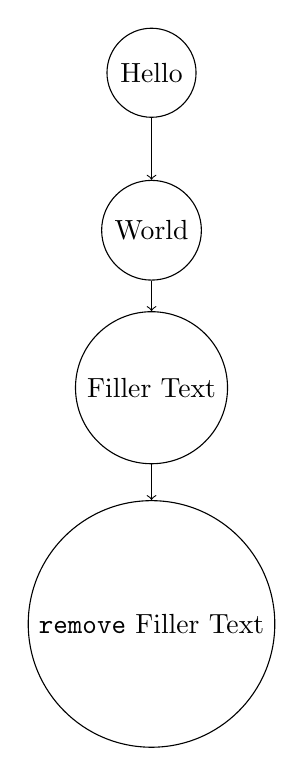
\begin{tikzpicture}
                    \node[circle, draw, minimum size=1cm] (A) at (0,0) {Hello};
                    \node[circle, draw, minimum size=1cm] (B) at (0,-2) {World};
                    \draw[->] (A) -- (B);
                    \node[circle, draw, minimum size=1cm] (C) at (0,-4) {Filler Text};
                    \draw [->] (B) -- (C);
                    \node[circle, draw, minimum size=1cm] (C2) at (0,-7) {\texttt{remove} Filler Text};
                    \draw [->] (C) -- (C2);
                \end{tikzpicture}
            }
        \end{column}
    \end{columns}

\end{frame}

\subsection{Branches and Merges}
\begin{frame}
    \frametitle{Branches and Merges}

    \begin{columns}
        \begin{column}{0.5\textwidth}
            \begin{itemize}[<+->]
                \item From our previous branching slide...
                \item We can swap between branches
                \item We can do work on branches
                \item We can merge branches
                \item Merging doesn't always work
            \end{itemize}
        \end{column}
        \begin{column}{0.5\textwidth}
            \resizebox{\textwidth}{!}{
                \begin{tikzpicture}
                    \node[circle, draw, minimum size=1cm] (A) at (0,0) {Hello};
                    \node[circle, draw, minimum size=1cm] (B) at (0,-2) {World};
                    \draw[->] (A) -- (B);
                    \node[gray, dashed, circle, draw, minimum size=1cm] (C) at (0,-4) {Filler Text};
                    \draw[gray, dashed, ->] (B) -- (C);
                    \node[circle, draw, minimum size=1cm] (D) at (3,-4) {Lorem Ipsum};
                    \draw[->] (B) -- (D);
                    \node[gray, dashed, circle, draw, minimum size=1cm] (C2) at (0,-7) {More filler text};
                    \draw[gray, dashed, ->] (C) -- (C2);
                    \node[] (LC2) at (-3, -7) {Branch 2};
                    \draw[->] (LC2) -- (C2);
                    \node[] (LB) at (-3, -2) {Branch 3};
                    \draw[->] (LB) -- (B);
                    \node[circle, draw, minimum size=1cm] (D2) at (3,-10) {merge};

                    \node[] (LD) at (6,-10) {\textbf{Branch 1}};
                    \draw[->] (LD) -- (D2);

                    \draw[->] (D) -- (D2);
                    \draw[->] (C2) -- (D2);
                \end{tikzpicture}
            }
        \end{column}
    \end{columns}
\end{frame}

\subsection{Collaborative Work}
\begin{frame}
    \frametitle{Collaborative Work}

    \begin{columns}
        \begin{column}{0.5\textwidth}
            \begin{itemize}[<+->]
                \item From our previous collaborative work slide...
                \item We can clone a repository from somewhere else
                \item We can push to a repository
                \item We can fetch from a repository
                \item We can merge the remote work in with our own
                \item We can use \textbf{pull} to combine these two processes
            \end{itemize}
        \end{column}
        \begin{column}{0.5\textwidth}
            \resizebox{!}{0.8\textheight}{
                \begin{tikzpicture}
                    % PERSON A
                    \node[circle, draw, minimum size=1cm] (A1) at (0,0) {Hello};
                    \node[circle, draw, minimum size=1cm] (B1) at (0,-2) {World};
                    \draw[->] (A1) -- (B1);
                    \node[gray, dashed, circle, draw, minimum size=1cm] (C1) at (0,-4) {Filler Text};
                    \draw[gray, dashed, ->] (B1) -- (C1);
                    \node[circle, draw, minimum size=1cm] (D1) at (3,-4) {Lorem Ipsum};
                    \draw[->] (B1) -- (D1);
                    \node[circle, draw, minimum size=1cm] (E1) at (3,-7) {dolor sit amet};
                    \draw[->] (D1) -- (E1);

                    % PERSON B
                    \node[circle, draw, minimum size=1cm] (A2) at (6,0) {Hello};
                    \node[circle, draw, minimum size=1cm] (B2) at (6,-2) {World};
                    \draw[->] (A2) -- (B2);
                    \node[gray, dashed, circle, draw, minimum size=1cm] (C2) at (6,-4) {Filler Text};
                    \draw[gray, dashed, ->] (B2) -- (C2);
                    \node[circle, draw, minimum size=1cm] (D2) at (9,-4) {Lorem Ipsum};
                    \draw[->] (B2) -- (D2);
                    \node[blue, circle, draw, minimum size=1cm] (F2) at (9,-7) {git is cool};
                    \draw[blue, ->] (D2) -- (F2);
                    \node[circle, draw, minimum size=1cm] (E2) at (12,-7) {dolor sit amet};
                    \draw[->] (D2) -- (E2);
                    \node[circle, draw, minimum size=1cm] (G2) at (10,-10) {merge};
                    \draw[->] (E2) -- (G2);
                    \draw[->] (F2) -- (G2);

                    % SERVER
                    \node[gray, dashed, circle, draw, minimum size=1cm] (A3) at (0,-8) {Hello};
                    \node[gray, dashed, circle, draw, minimum size=1cm] (B3) at (0,-10) {World};
                    \draw[gray, dashed, ->] (A3) -- (B3);
                    \node[gray, dashed, circle, draw, minimum size=1cm] (C3) at (0,-12) {Filler Text};
                    \draw[gray, dashed, ->] (B3) -- (C3);
                    \node[gray, dashed, circle, draw, minimum size=1cm] (D3) at (3,-12) {Lorem Ipsum};
                    \draw[gray, dashed, ->] (B3) -- (D3);
                    \node[gray, dashed, circle, draw, minimum size=1cm] (E3) at (3,-15) {dolor sit amet};
                    \draw[gray, dashed, ->] (D3) -- (E3);
                    \node[gray, dashed, circle, draw, minimum size=1cm] (F3) at (6,-15) {git is cool};
                    \node[gray, dashed, circle, draw, minimum size=1cm] (G3) at (4,-18) {merge};
                    \draw[gray, dashed, ->] (D3) -- (F3);
                    \draw[gray, dashed, ->] (E3) -- (G3);
                    \draw[gray, dashed, ->] (F3) -- (G3);
                \end{tikzpicture}
            }
        \end{column}
    \end{columns}

\end{frame}

\end{document}
